\section{Research Background}

Biometrics technology is a technology that identifies or verifies individuals based on their physiological characteristics such as fingerprints, face, iris, or behavioral characteristics such as voiceprints and handwritten signatures. This technology is widely used in security authentication, financial transactions, access control systems and other security areas \cite{12} for personal identification or verification. In the identification scenario, the system will identify the user profile already in the system database based on the physiological or behavioral characteristics provided by the user. This scenario is applicable to fingerprint, iris personal identification, etc. Secondly, in the verification scenario, the user needs to provide the system with verified identity and characteristic information, and the system will judge whether the current user is the declared user based on the stored characteristic information and the information currently provided by the user, which is applicable to the scenarios of declaring personal identity and providing personal characteristic information, such as the unlocking of smart phones and international border crossing.

Handwritten signature is a more important individual behavioral characteristic in daily life, and as the main characteristic for verifying personal identity in legal, financial, administrative and other fields, because it cannot be intruded during the collection process, handwritten signature is also regarded as one of the main characteristics of many technologies for verifying personal identity. Handwritten signatures produce different writing styles, such as regular and cursive, depending on the individual's writing habits. Even with the passage of time, the personal writing style may change, and the signature (defined as Query) provided by the user after a certain period of time may differ from the reference signature (defined as Reference) previously entered into the system. As a result, there will be some difficulties in comparing the verification of the user's handwritten signature, for example, there will be differences in the angle of the bending strokes, the length of the straight line, and the hook at the end of each character on the personal signature. As mentioned above, the handwritten signature may be slightly different in the end due to different writing habits of individuals. Therefore, in order to obtain the identity authority of a certain user, some people will maliciously forge handwritten signatures in order to pass the security and privacy checking system, or even practice for a long period of time in order to achieve a handwritten signature of a similar style as that of a certain user. As a result, academics have launched a series of studies on handwritten signature verification, hoping to design a relevant model to help relevant staff to more efficiently complete the process of more repetitive handwritten signature verification work, so that more staff to participate in the core work.

In academia, handwritten signature verification is categorized into two types, offline and online, depending on the data collection route. The collection process of offline handwritten signatures is obtained after the user's writing process on paper; online handwritten signatures are collected by using a digitizing station, and the collected handwritten signature images may be affected by the equipment, such as the position of the pen, tilt, and pressure, etc. \cite{2}. In addition to the different data collection routes are categorized into different types of handwritten signature verification, scholars have defined two types of branching tasks, Writer-Independent (WI) and Writer-Dependent (WD) to evaluate the model algorithms. The WI task is needed to input a pair of handwritten signature image to the model structure, based on the features extracted from the reference signature and the query signature so as to determine whether the query signature is forged or not. the WD task adds the author id to the input of the WI task, and uses the corresponding author classifier according to the author id in order to determine whether the query signature is forged or not. These two branching tasks, although both output the label category of query signatures (genuine or forged) at the end, can reflect the different performance of the model to different degrees. The WI task focuses on learning the global characteristics of the signature population, does not need to learn a separate writer classifier for each user, and has the excellent extensibility of not requiring re-training for new users, and at the same time can reflect the generalization and discriminative ability of the model. The WI task focuses on learning the global features of the signature group, does not need to learn an writer classifier for each user individually, has excellent scalability without re-training for new users, and can reflect the model's generalization and discriminative ability; the WD task additionally trains an writer classifier for each user individually, which can take into account the high accuracy of different styles of signatures of individual writers that are still considered to be real signatures, but needs to collect a sufficiently large number of samples for each user, with a high cost of training and a weak generalization ability. Thus the WI and WD tasks can reflect the overall performance of the model to different degrees, and the model performance is comprehensively evaluated according to the evaluation indexes of the two tasks.

With the development of the level of technology, the field of artificial intelligence has been able to generate fake pictures based on the sample images and keywords provided by the user, and it is difficult for normal people to identify the real and fake with the naked eye. Therefore, there will be part of the artificial generation of forged signature behavior, so as to achieve the fake to pass the verification of the security system, resulting in personal privacy, property invasion, theft and other dangerous consequences. Relying on manual power to verify will have certain social risks and judgment errors, so the study of offline handwritten signature verification, to a certain extent, can reduce the risk of forged signatures through the verification of the relevant algorithmic models to help minimize the error of manual verification, so as to better ensure personal privacy and property security.

\section{Research Motivation and Importance}

This work focuses on the offline handwritten signature verification task, which is essentially a derivative branch of an image categorization task. Unlike the traditional image categorization task, the offline handwritten signature verification task requires the input of a reference and query pair of signature image samples, and the WD task needs to additionally input an writer id in order to train an writer-independent classifier. The offline handwritten signature verification model will extract relevant image features based on the input reference and query signature images, and compare the features to output genuine or forged category labels. Thus the task is challenging and innovative, the design of the model or algorithm architecture not only needs to consider the criticality of the model to extract a pair of image features, the model architecture of the isotropic dual-stream will directly affect the criticality of the features extracted from the reference signature and query-signature images, and once the extracted features don't have so important information, it will lead to a drastic decrease in the model's ability to make judgments. At the same time, due to the definition of the WI and WD tasks and the real-life application scenarios, it is required to have a high accuracy rate and generalization ability to prevent personal privacy and property infringement, but also to enhance the demand for model performance, which makes the design and experimentation of the offline handwritten signature verification model a very challenging image task.

In the design of offline handwritten signature verification model, it is divided into two parts: feature extractor and writer classifier for WD task. In the past researches of scholars, most of them manually design the image feature extraction method based on the data cluster features such as sample distribution, and take the traditional machine learning method to determine whether the signature is forged or not \cite{12}, such as taking the distance between the features or SVM to determine whether the signature is forged or not. But this manually designed features have the defects of specific data clusters, it must require the data set of the writer's signature style uniformity, subtle differences will be as outliers leading to the traditional machine learning methods to determine the accuracy of the decline in the accuracy of the work, but the actual production work is required to have these certain differences in the tolerance of the degree of the work, so this method of taking the artificial design of the extracted features is gradually phased out. Scholars hope to have an image feature extractor that focuses more on a certain part of the image and does not need to intervene many times. With the rapid development of deep learning in the past six years, convolutional neural network (CNN) with shared parameters for local field of view operations has achieved good results in traditional image classification tasks such as MNIST, ImageNet, and compared with the traditional machine learning methods, the accuracy and generalization ability of CNN is even better than that of traditional machine learning methods. The accuracy and generalization ability of CNNs have been further verified in comparison with traditional machine learning methods. As a result, scholars in the field of handwritten signature verification have introduced CNN as a feature extractor, and experiments have proved that the accuracy and generalization ability of this approach has made a great breakthrough compared with previous methods \cite{11}.

Even though CNN's ability to extract image features is outstanding, its core idea of convolutional kernel operation has a certain local field of view reinforcement learning ability, which can focus on the local features of the image; however, for handwritten signatures not only need to pay attention to the degree of the corners of the font strokes, but also need to pay attention to the overall style of the signature image, fonts, and other factors, which may result in the case of the signature of the same writer in a different location, so CNN as a feature extractor still has some defects. With the development of the field of natural language processing, the appearance of Transformer \cite{36} with global feature learning attracted the attention of scholars, and then scholars in the field of image introduced the Encoder-Decoder architecture of Transformer to experiment on the image classification task \cite{4}, and the experiments proved that the performance of this approach is better than CNN's feature extractor in the case of convergence of model parameters. It is proved that this approach has better performance than CNN's feature extractor in the case of model parameter convergence, but the conditions for training to achieve model parameter convergence are more demanding, because Transformer's attention mechanism needs to learn the whole image, whereas CNN adopts the way of sharing parameters to learn the local features of the image, so that model convergence can be achieved faster, but the generalization ability is poorer in practice, and we need to keep fine-tuning the dataset in order to achieve higher model performance. However, in practice, the generalization ability is poor and the dataset needs to be constantly fine-tuned to achieve higher model performance. As a result, CNN is derived as Backbone to extract multi-channel feature maps, which are flattened as feature vectors and entered into the Transformer for global attention feature operation \cite{9}, so as to achieve the multi-channel feature maps in the absence of overall information, and then strengthen the characteristics of the overall information through the Transformer's attention mechanism, which is proved by experiments to be more effective in learning image features and modeling. Experiments have proved that this approach can learn image features more effectively, and the model thus achieves better accuracy and generalization ability. In summary, the CNN+Transformer style model architecture has become the mainstream framework in the image field in recent years, and it has also been introduced in offline handwritten signature verification tasks and experiments have proved that this style of model architecture has good model performance \cite{9}, so the offline handwritten signature verification model based on Transformer proposed in this work is also a CNN+Transformer style model architecture. Transformer style model architecture, in line with the development trend of this field in deep learning in recent years, and on this basis, multi-scale fusion features are added, in order to meet the growing requirements of high-definition image resolution at the same time, to learn the signature image font stroke corners and other features at multiple scales, to make up for the shortcomings of the multi-channel feature maps in terms of the scale after the CNN. In the final output classification stage, unlike the traditional image classification task, the model proposed in this work will collect the features from the previous modules in the final output features, and perform overall stitching for category label prediction or model training, which has been proven to be effective \cite{41}. The challenge of the research is how to effectively use multi-scale fusion features for category prediction and model training, this way of training and prediction using the overall model features can better train the model weights of each part in a holistic manner, and the model training to the convergence stage will surpass most of the previous deep learning model architectures, which is a novel idea for the related fields to integrate the feature approach of convolutional neural networks and attention mechanisms. For related fields, it provides a novel idea to integrate the features of convolutional neural network and attention mechanism, which provides a certain design idea for the subsequent more concise fusion module; on the contrary, this approach will increase the computational reasoning pressure of the equipment and the cost of model training, and it needs to be proved by various experiments that this approach is effective.

\section{Research Objects}

The Offline Signature Verification TransFormer (OSVTF) structure proposed in this work, as a whole, is a model designed based on the idea of siamese networks, as shown in Fig. \ref{fig:overview}.

\begin{figure}[htbp]
    \begin{center}
        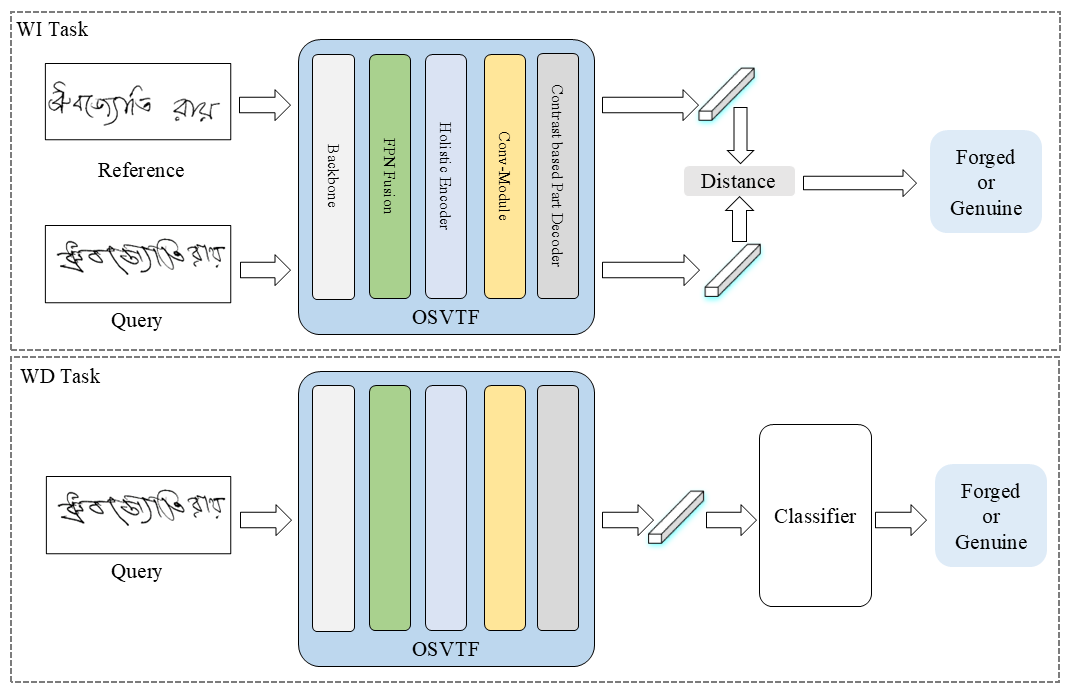
\includegraphics[scale=0.5]{figure/overview.png}
    \end{center}
    \caption{OSVTF overview}
    \label{fig:overview}
\end{figure}

The core idea of the siamese network is two sub-networks with shared weights that accept two inputs and output two feature vectors, and subsequently calculate the similarity using a distance function \cite{10}. In the WI and WD tasks of offline handwritten signature verification, a pair of images of the inputreference and query signatures are input, so the overall architecture is referred to TransOSV \cite{41}, based on which the backbone and FPN Fusion modules are added, and the Encoder, Conv-Module, and Decoder sections are subjected to a The Encoder, Conv-Module and Decoder parts are optimized and adjusted in a series of ways, which are more conducive to the change and learning of the features of each part, and the experimental part is needed to confirm that these modules can improve the model's ability of judging forged signatures and generalization ability in different scenarios.

In the overall research plan and experiments, the two general directions of WI and WD are still adopted to evaluate the performance and quality of the model as a whole, based on which the multi-channel feature maps of CNN and the attention mechanism of Transformer will be visualized, and we need to pay attention to whether these modules are able to better grasp some of the important feature information of the image in the image feature learning. In addition, there are many ways of fusion of multi-scale features, such as Mask R-CNN \cite{13} takes the feature pyramid network style (FPN-Style) \cite{23}, this kind of fusion includes, but is not limited to, mean accumulation, direct summation, and splicing, so the follow-up will be to train the model of these fusion methods with the control variables in order to get the best performance of fusion of multi-scale feature maps way. In addition, the previous twin network approach is to calculate the similarity based on the distance function in order to complete the related tasks, whether this approach can still be effective after the addition of multi-scale fusion features requires some verification, this work will refer to the traditional image classification task of the CNN processing classification approach, the addition of a global average pooling layer as a classifier to classify the features label prediction, in order to determine whether it would be outperform the previous distance similarity judgment.

In summary, this work will be divided into three parts of the research phase: 1. Initially, the OSVTF model architecture will be trained in the model cycle to verify whether the optimized and adjusted scheme of multi-scale features and models can be improved on the original architecture; 2. For the multi-scale fusion method of the FPN Fusion module, a small fine-tuning training will be taken on the basis of the first phase of the control variable method for the model, and the best multi-scale feature fusion method will be selected. The best multi-scale feature fusion method; 3. For the WD task, a global average pooling classifier is added in the final classifier stage, which is compared with the previous method of distance similarity prediction for offline handwritten signature verification, so as to judge the advantages and disadvantages of the two classifiers, and a better classifier is adopted for experiments in the WD task to verify whether it works.
